\chapter{Espaços e Funções Mensuráveis}

Nesta seção, apresentaremos os conceitos que fundamentam a teoria da medida. Trataremos, especificadamente, de $\sigma$-álgebra, espaços mensuráveis e funções mensuráveis. 
Embora estejamos assumindo que o leitor já esteja familiarizado com a teoria de conjuntos, faremos algumas observações sobre notação de alguns conjuntos com o objetivo de cessar o maior número de dúvidas.
Iniciaremos definindo \sigal para que possamos construir espaços mensuráveis.
Em seguida, abordaremos as funções mensuráveis.
Todas as definições e resultados aqui explorados, bem como nas demais seções,  tiveram como principal fonte o livro \textit{The Elements of Integration and Lebesgue Measure}\footnote{Em português: Os Elementos da Integração e Medida de Lebesgue.} do autor Robert G. Bartle.

\section{O Conceito de \sigal}
% Definição de Sigma álgebra
Para que possamos estabelecer uma \enquote{medida} precisamos de um ambiente que permita ser \enquote{medido}. 
Criamos um ambiente como este adicionando uma estrutura algébrica específica em um conjunto.
Tal estrutura recebe o nome de $\sigma$-álgebra e é definida em \cite{bartle} da seguinte forma:

\begin{env}{Definição}
\label{def:sigma-algebra}
\index{$\sigma$-álgebra}
    Seja $X$ um conjunto não vazio. Uma família $\mathcal{C}$ de subconjuntos de $X$ é dita uma \sigal se as seguintes condições são atendidas:
    \begin{enumerate}[label*= (\roman*)]
        \item $\varnothing$ e $X$ são elementos de $\mathcal{C}$;     
        \item Se um elemento $A \in \mathcal{C}$, então $A^c \in \mathcal{C}$
        \footnote{Em todo o texto, $X^c$ significa o complementar do conjunto $X$.};
        \item Se $(A_j)$ é uma sequência
        \footnote{
        	\enquote{%
        	[...] uma sequência 
        	$x = (x_n)_{n \in \N} = (x_1, x_2,..., x_n,...)$ de elementos de um conjunto
        	$X$ é uma função $x: \N \to X$, onde o valor $x(n)$ é indicado pelo símbolo $x_n$ e chama-se o n-ésimo termo da sequência%
        	} \cite[p.25]{elon}.
    	} de elementos de $\mathcal{C}$, 
        então $\displaystyle \bigcup_{j = 1}^\infty A_j \in \mathcal{C}$.
        \vspace{-0.2cm}
        \index{Sequência}
    \end{enumerate}
\end{env}

Com isso, um par ordenado $(X, \mathcal{C})$  constituído de um conjunto $X$ e uma $\sigma$-álgebra sobre $X$ é chamado, pelo mesmo autor, de  \textbf{espaço mensurável}.
Além disso, cada elemento deste espaço é chamado de conjunto $\mathcal{C}-$mensurável.
Quando não houver confusão ou quando a \sigal estiver fixada, dizemos simplesmente que cada elemento é um conjunto mensurável. 
Observe que a terceira condição da \ref{def:sigma-algebra} nos diz que a união enumerável
%
\footnote{Para esse tipo de conjunto, utilizaremos a definição \enquote{Um conjunto $X$ diz-se \textit{enumerável} quando é finito ou quando existe uma bijeção $f : \N \to X$.} \cite[p.48]{elon}}
%
é um elemento da $\sigma$-álgebra.
Logo, para um número finito $A_1, A_2, ..., A_n$ com $n \in \N$ de elementos $\cc$-mensuráveis de uma \sigal $\cc$, a união $\displaystyle \bigcup_{j \in I_n} A_j$ também será um elemento $\cc$-mensurável.

\begin{env}{Observação}
	Em todo o texto, indicaremos por $I_n$ o conjunto dos $n$ primeiros números naturais, isto é, $I_n = \{k \in \N; 1 \leq k \leq n\}$.
\end{env}
% Exemplos de Sigmas Algebras 
\begin{env}{Exemplo}
	\label{ex:Primeiro Exemplo Sigma Algebra}
    Seja $X = \{-1,0,1\}$. Se considerarmos $\mathcal{C} = \{\varnothing, X, \{0\}, \{-1,1\}\}$, temos que $(X, \mathcal{C})$ é um espaço mensurável.
    \vspace{-0.2cm}
\end{env}
%
\begin{env}{Exemplo}
	\label{ex:sigma-trivial}
	Seja $X$ um conjunto qualquer.
	O conjunto $\mathcal{C}_1 = \{\varnothing, X\}$ é uma \sigal de $X$.
	De fato, podemos observar que, nesse exemplo, todas as condições impostas na  \ref{def:sigma-algebra} são atendidas de maneira trivial, pois 
	$\varnothing$ e $X$ são todos os elementos de $\mathcal{C}_1$. 
	Assim,  $(X, \mathcal{C}_1)$ é um espaço mensurável.
\vspace{-0.2cm}
\end{env}

	Perceba que a \ref{def:sigma-algebra} não nos diz que uma \sigal de um conjunto é única.
Realmente, não é. 
Assim, um conjunto pode gerar espaços mensuráveis diferentes a depender da \sigal adotada.
Para evidenciar essa percepção, observe o exemplo a seguir:

\begin{env}{Exemplo}
	\label{ex:sigma-subconjuntos}
	Seja $X$ conforme o exemplo anterior.
	Considere, agora, o conjunto \linebreak $\mathcal{C}_2 = \{ A; \ A \subset X\}$, ou seja, o conjunto formado por todos os subconjuntos do conjunto $X$
	%
	\footnote{O conjunto $\cc_2$ também é chamado de conjunto das partes de $X$ e, as vezes, é representado por $\mathcal{P}(X)$.}.
	Sabemos que $\varnothing \subset X$ e $X \subset X$. 
	Assim, $\varnothing, X \in \mathcal{C}_2$. 
	Se tomarmos um conjunto $A \subset \mathcal{C}_2$, então $A^c = X - A$ por definição.
	Ou seja, $A^c$ é formado por elementos que estão todos em $X$ caracterizando-o um elemento de $\mathcal{C}_2$.
	Da mesma forma, se tomarmos uma sequência $(A_j)$ de elementos de $\mathcal{C}_2$, a reunião 
	$\displaystyle \bigcup_{j = 1}^\infty A_j$ é composta por elementos de $X$.
	Logo,  $\displaystyle \bigcup_{j = 1}^\infty A_j \in \mathcal{C}_2$.
	Com isso, $\mathcal{C}_2$ também é uma \sigal de $X$ e o par $(X, \mathcal{C}_2)$ é um espaço mensurável que, por sua vez, é diferente do espaço $(X,\mathcal{C}_1)$.
	\vspace{-0.2cm}
\end{env}

Os exemplos apresentados acima são todos de conjuntos que são uma \sigal de um conjunto $X$ arbitrário.
Por definição, o conjunto $\mathcal{C}$ é composto de subconjuntos do conjunto $X$. 
Será que se construirmos $\cc_3$ um conjunto que contenha $\varnothing$ e $X$ e outros subconjuntos do conjunto $X$ tomados aleatoriamente teremos $(X,\cc_3)$ um espaço mensurável? A resposta é negativa e para convencê-lo disso, mostraremos o seguinte contra-exemplo.

%Contra Exemplo
\begin{env}{Contraexemplo}
    Seja $X = \{x,y,z\}$. O conjunto $\mathcal{C} = \{\varnothing, X, \{x\}, \{y\}, \{z\}\}$ não é uma \sigal de $X$.
    Sem dúvida, $\varnothing, X \in \mathcal{C}$. 
    Entretanto, perceba que $\{x\} \in \mathcal{C}$, mas $\{x\}^c \notin \mathcal{C}$.
    De fato, 
    $
    \{x\}^c
    =\{x,y,z\} 
    -\{x\} 
    = \{y,z\}.
    $
    Mas $\{y,z\} \notin \mathcal{C}$.
    Assim, a segunda condição da \ref{def:sigma-algebra} não é satisfeita, impossibilitando que $\mathcal{C}$ seja uma \sigal de $X$.
    \vspace{-0.2cm}
\end{env}

A proposição adiante nos mostra como podemos induzir uma \sigal com um conjunto fixado,  não vazio, em um conjunto.
\begin{env}{Proposição}
\label{prop:sigma-complementar}
    Seja $X$ e $A$ dois conjuntos quaisquer com $A \neq \varnothing$.
    Se $A \subset X$, então o conjunto 
    $\mathcal{C}=\{\varnothing, X, A, A^c\}$ é uma \sigal de $X$.
\end{env}

\begin{prova}
    Perceba que as condições \textit{(i)} e \textit{(ii)} da  \ref{def:sigma-algebra} são satisfeitas pela forma que o conjunto  $\mathcal{C}$ foi construído. Para verificar a última condição, basta perceber $A \cup A^c = X$. Portanto, $\mathcal{C}$ é uma \sigal de $X$ para qualquer que seja $ \varnothing \neq A \subset X$.
\end{prova}

Perceba que a \ref{prop:sigma-complementar} generaliza o \ref{ex:Primeiro Exemplo Sigma Algebra}. Além disso, possibilita uma criação de uma \sigal em um conjunto qualquer não vazio.
Por exemplo, considere $X = \N$.
Tome $P =\{2k; \ k \in \N\}$ e $I = \{2k - 1;\ k \in \N\}$.
Como $P^c = I$, então $\mathcal{C} = \{\varnothing, \N, P, I\}$ é uma \sigal de $\N$ pela proposição anterior.
Note que a  \ref{def:sigma-algebra} trata apenas da reunião enumerável de elementos da $\sigma$-álgebra. 
Nosso interesse, agora, é investigar se conseguirmos propriedades análogas para a operação de interseção. 
Iniciaremos verificando o comportamento de interseção de elementos de uma \sigal com a seguinte proposição:
% Propriedades de Interseção 

\begin{env}{Proposição}
\label{prop:interseção-elementos-sigmas}
    Seja $(X, \cc)$ um espaço mensurável.
    Se $(A_j)$ é uma sequência  de conjuntos $\mathcal{C} $-mensuráveis, então $\displaystyle \bigcap_{j = 1}^\infty A_j$ é um elemento $\mathcal{C}$-mensurável.
\end{env}
\begin{prova}
    Se $A_j \in \mathcal{C}$ para todo $j \in \N$, então cada complementar $A_j^c \in \mathcal{C}$, pois $\mathcal{C}$ é $\sigma$-álgebra. 
    Assim, $(A_j^c)$ forma uma sequência de conjuntos $\mathcal{C}$-mensuráveis acarretando que 
    $\displaystyle \bigcup_{j = 1}^\infty A_j^c \in \mathcal{C}$. 
    Segue, pelas \textit{Leis de De Morgan}
    \footnote{O enunciado e as demonstrações dessas leis podem ser encontrados em \cite[p.26]{elon}}, que 
    $$
    \displaystyle \bigcup_{j = 1}^\infty A_j^c 
    = \left(\displaystyle \bigcap_{j = 1}^\infty A_j\right)^c
  	$$
	Logo, $\left(\displaystyle \bigcap_{j = 1}^\infty A_j\right)^c \in \mathcal{C}$ implica $\displaystyle \bigcap_{j = 1}^\infty A_j \in \mathcal{C}$, pois $(X^c)^c = X$, para qualquer conjunto $X$.
	Portanto, $\displaystyle \bigcap_{j = 1}^\infty A_j$ é um elemento $\mathcal{C}$-mensurável.
\end{prova}

\begin{env}{Proposição}
	\label{prop: provar que a menor sigma algebra e algebra}
	Dada uma coleção de conjuntos $\mathcal{T}$ de subconjuntos de $X$, a interseção de todas as $\sigma$-álgebras que contêm $\mathcal{T}$ é uma $\sigma$-álgebra.
\end{env}
\begin{prova}
	Seja $\Sigma$ a interseção de todas as $\sigma$-álgebras $\cc$ que contêm $\mathcal{T}$, isto é, 
	$\Sigma = \displaystyle \bigcap_{\mathcal{T} \in \cc } \cc$.
	Pela \ref{def:sigma-algebra}, $\varnothing, X \in \cc$ para qualquer $\cc$ $\sigma$-álgebra.
	Logo, $\varnothing, X \in \Sigma$.
	Tome um elemento $A \in \Sigma$.
	Assim, $A \in \cc$ para toda $\cc$ que contêm $\mathcal{T}$.
	Ou seja, $A^c \in \cc$ para toda \sigal $\cc$. 
	Logo, $A^c \in \Sigma$.
	Analogamente, tomando uma sequência de elementos $(A_j) \in \Sigma$, vemos que $A_j \in \cc$ para todo $j \in \N$. 
	Dessa forma, $\displaystyle \bigcap_{j \in \N} A_j \in \cc,\ \forall \cc$ acarretando que $\displaystyle \bigcap_{j \in \N} A_j \in \Sigma$.
	Portanto, $\Sigma$ é uma $\sigma$-álgebra.
\end{prova}

\begin{env}{Definição}
	\label{deff: sigma algebra gerada}
	\index{$\sigma$-álgebra! gerada}
	Dada uma coleção de conjuntos $\mathcal{T}$ de subconjuntos de $X$ e $\cc$ uma $\sigma$-álgebra que contêm $\mathcal{T}$, dizemos que
	$
	\Sigma = \displaystyle \bigcap_{\mathcal{T} \in \cc } \cc
	$
	é a $\sigma$-álgebra gerada por $\mathcal{T}$
	\footnote{Também pode ser definida como a \textit{menor} $\sigma$-álgebra de $\mathcal{T}$ sendo a noção de \enquote{menor} trazida por meio da ordem parcial gerada pela relação de inclusão entre conjuntos.}.
\end{env}

Considere a \sigal apresentada na \ref{prop:sigma-complementar}. 
Qualquer outra \sigal $\mathcal{F}$ que tiver $A$ como elemento, conterá $\mathcal{C}$.
Logo, $\cc$ é a álgebra gerada por $A$.
Sabendo que a menor \sigal é gerada por meio de intersecções é natural questionarmos se a interseção entre \sigals ainda é uma \sigal de $X$.
Responderemos à esta pergunta com a proposição adiante.
\vspace{-0.1cm}
%Interseção de Sigmas algebras
\begin{env}{Proposição}
\label{prop:interseção-sigmas-quaisquer}
    Sejam $X$ um conjunto não vazio e $\mathcal{F}$ uma família arbitrária de conjuntos.
    Se $\cc_A$ é uma \sigal para todo $A \in \mathcal{F}$, então
    $
    \displaystyle \cc = \bigcap_{A \in \mathcal{F}} \cc_A$ é uma $\sigma$-álgebra de $X$. 
\end{env}
\begin{prova}
    Como $\cc_A$ é uma \sigal para todo $A \in \mathcal{F}$, então 
    $\varnothing, X \in \cc$.
    Tome um $E \in \cc$. 
    Assim, $E \in \cc_A\ \forall\  A \in \mathcal{F}$.
    Logo, $E^c \in \cc_A\ \forall\  A \in \mathcal{F}$ pela \ref{def:sigma-algebra}.
    Com isso, $E^c \in \cc$.
    Por fim, tome uma sequência de elementos $(E_j)$ com $E_j \in \cc$ para todo $j \in \N$.
    Desta forma, $E_j \in \cc_A$ para todo $A \in \mathcal{F}$ e $j \in \N$.
    Daí, pela definição de $\sigma$-álgebra, 
    $\displaystyle\bigcup_{j \in \N} E_j \in \cc_A \ \forall\ A \in \mathcal{F}$.
    Disso, $\displaystyle \bigcup_{j \in \N} E_j \in \cc$.
    Portanto, $\cc$ é uma $\sigma$-álgebra.
\end{prova}


Note que há uma diferença gritante entre a \ref{prop:interseção-elementos-sigmas} e \ref{prop:interseção-sigmas-quaisquer}.
A primeira trata de conjuntos mensuráveis de uma \sigal e a outra refere-se à \sigals de um conjunto $X$.
Além disso, perceba que até aqui trabalhamos o conceito de \sigal de maneira abstrata sendo utilizada em um conjunto qualquer. 
Trataremos, agora, de uma \sigal extremamente importante e específica para o conjunto $\R$ dos números reais.

% Álgebra de Borel
\begin{env}{Definição}
\label{def:algebra-borel}
    Seja $X = \R$. Definimos como a \sigal de Borel, e representaremos por $\borel$, a \sigal gerada por todos os intervalos abertos $(-\infty,x)$ com $ x  \in \R$. 
    \index{$\sigma$-álgebra! de Borel}
\end{env}

Os elementos da \sigal de Borel recebem o nome de Borelianos.
Esta \sigal é extremamente relevante para os estudos de medida e integração e pode ser definida de várias formas diferentes, mas todas são equivalentes.
Isso quer dizer que $(-\infty, x)$ não é a única forma dos elementos de $\borel$. 
De fato, se  $(-\infty, x) \in \borel$, então $(-\infty, x)^c \in \borel$ só que $(-\infty, x)^c = [x, +\infty$).
Assim, poderíamos  definir  $\borel$ por meio de intervalos do tipo $[x, +\infty)$.
Em particular, poderíamos ter definido a $\borel$ por meio da \sigal gerada por intervalos do tipo $(a,b)$ com $a,b \in \R$. 

Antes de provarmos este fato, observe que podemos decompor intervalos reais como a união de outros intervalos reais. 
Por exemplo, utilizando a reta real, podemos representar intervalo $(-\infty, b)$ da seguinte maneira\\

% Imagem da decomposição de intervalos.
\begin{figure}[h!]
	\centering
	\Caption{\label{fig:intervalo de infinito ate b} Intervalo $(-\infty, b)$ }	
	\UECEfig{}{
	    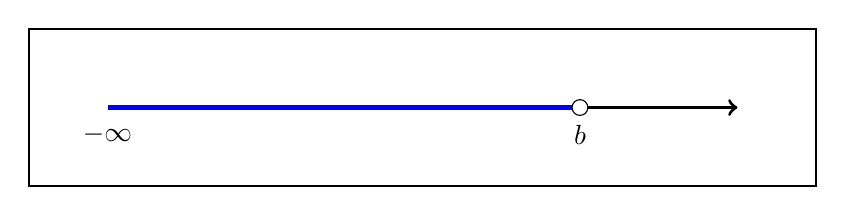
\begin{tikzpicture}
	    	\draw[thick] (-5, -1) rectangle (5, 1);
              % Eixo horizontal
              \draw[->, very thick] (-4,0) -- (4,0);
            
              % Linha vertical para representar x
              \draw[dashed] (2,-0.1) -- (2,0.1);
              % Rótulo para -∞
              \node[below] at (-4,-0.1) {$-\infty$};
              % Rótulo para x
              \node[below] at (2,-0.1) {$b$};
              % Desenhar o intervalo aberto (-∞, x)
              \draw[ultra thick, blue] (-4,0) -- (2,0);
              % Adicionar a bolinha aberta em x
              \draw[fill=white] (2,0) circle (0.1);
        \end{tikzpicture}
	}{
	    \Fonte{Elaborado pelo autor}
	}	
\end{figure}
Se tomarmos um $a \in \R$ fixo, com $a<b$, então a decomposição do intervalo $(-\infty, b)$ pode ser expressa por meio da união dos intervalos $(-\infty, a]$ e $(a,b)$, onde estão representados na figura a seguir pelas cores azul e vermelha, respectivamente.\\
\begin{figure}[h!]
	\centering
	\Caption{\label{fig:boreliano-decomposto} Representação de uma decomposição do intervalo $(-\infty, b)$ na reta real}	
	\UECEfig{}{
        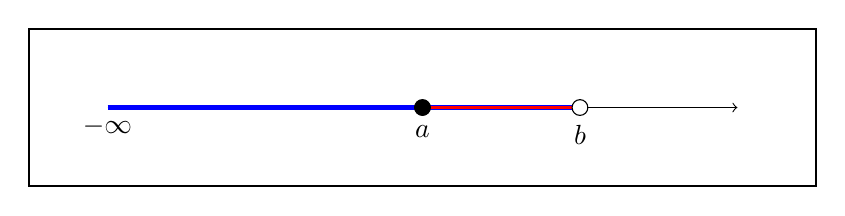
\begin{tikzpicture}
        	\draw[thick] (-5, -1) rectangle (5, 1);
              % Eixo horizontal
              \draw[->] (-4,0) -- (4,0);
              % Linha vertical para representar x
              \draw[dashed] (2,-0.1) -- (2,0.1);
              % Rótulo para -∞
              \node[below] at (-4,0) {$-\infty$};
              % Rótulo para x
              \node[below] at (2,-0.1) {$b$};
                
              % Rótulo para a
              \node[below] at (0,-0.1) {$a$};
              
              % Desenhar o intervalo aberto (-∞, x)
              \draw[ultra thick, blue] (-4,0) -- (2,0);
            
              % Desenhar o intervalo aberto (a,b)
              \draw[very thick, red] (0,0) -- (2,0);
              
              % Adicionar a bolinha aberta em x
              \draw[fill=white] (2,0) circle (0.1);
              \draw[fill=black] (0,0) circle (0.1);
        \end{tikzpicture}
	}{
	    \Fonte{Elaborado pelo autor}
	}	
\end{figure}\\
A decomposição de intervalos reais pela união de outros é relevante para mostrar a seguinte equivalência sobre a \sigal de Borel.\\
\begin{env}{Teorema}
\label{teo:equiv-borel}
    Uma \sigal é de Borel  se, e somente se, é gerada por intervalos do tipo $(a,b)$ com $a,b \in \R$.
    \vspace{-0.2cm}
\end{env}
\begin{prova}
   Suponha que $\borel$ seja a $\sigma$-álgebra de Borel. 
   Sejam $a$ e $b$ números reais, com $a<b$.
   Como $a + \dfrac{1}{n} \in \R$ para todo $n \in \N$, temos que o intervalo
   $
   \left(-\infty, a + \dfrac{1}{n}\right) \in \borel$ para todo $n \in \N
   $.
   Segue, pela \ref{prop:interseção-elementos-sigmas}, que
   $
   \displaystyle \bigcap_{n = 1}^\infty \left(-\infty, a+ \dfrac{1}{n}\right) \in \borel
   $.
   Com isso, afirmamos que a interseção de todos os intervalos $\left(-\infty, a + \dfrac{1}{n}\right)$ é igual ao intervalo $(-\infty, a]$.
   De fato,
   \begin{align*}
	x \in \bigcap_{n \in \N} \left(-\infty, a + \dfrac{1}{n}\right)
   	\Leftrightarrow & x \in \left(-\infty, a + \dfrac{1}{n}\right), \ \forall \ n \in \N\\
   	\Leftrightarrow & x < a + \dfrac{1}{n}, \ \forall \ n \in \N\\
   	\Leftrightarrow & \dlim_{n \to +\infty} x \leq \dlim_{n \to +\infty} \left(a + \dfrac{1}{n}\right)\\
   	\Leftrightarrow & x \leq a\\
   	\Leftrightarrow & x \in (-\infty, a].
   \end{align*}
	Logo, $(-\infty, a] \in \borel$ acarretando que $(a, +\infty) = (-\infty, a]^c \in \borel$.
	Observe que podemos decompor $(-\infty, b) = (-\infty,a] \cup (a, b)$ enquanto que $(a, +\infty) = (a, b) \cup [b, +\infty)$.
	Desta forma, vemos que $(-\infty, b) \cap (a, +\infty) = (a,b)$. 
	Como $(-\infty, b)$ e $(a, +\infty)$ são elementos de $\borel$, segue pela 
	\ref{prop:interseção-elementos-sigmas} que $(a,b) \in \borel$.
	Com isso, $\borel$ pode ser gerada por intervalos do tipo $(a,b)$ com $a,b \in \R$.
   
	Suponha, reciprocamente, que $\mathcal{C}$ é uma \sigal de $\R$ gerada por $(a,b)$ com $a,b \in \R$.
	Como $(a, b) \in \cc$, então $(a,b)^c \in \cc$, por definição de $\sigma$-álgebra.
	Logo, $(-\infty,a])\cup [b,+\infty) \in \cc$.
	Além disso, os conjuntos $A_n = (-n, a)$ são todos elementos de $\mathcal{C}$ para qualquer $n \in \N$.
	Segue, pela  \ref{def:sigma-algebra}, que 
	$\displaystyle \bigcup_{n = 1}^\infty (-n,a) \in \mathcal{C}$.
	Só que $\displaystyle \bigcup_{n = 1}^\infty (-n,a) = (-\infty, a)$. 
	Disso, $(-\infty, a)\cap \left\{(\infty,a])\cup [b,+\infty)\right\} \in \cc$. Portanto,  $(-\infty, a) \in \cc$ como queríamos.
	%% FFALTA PROVAR AINDA DIREITINHO.
\end{prova}

\section{Funções Mensuráveis}
Agora que já estamos familiarizados com os conceitos de \sigal e espaços mensuráveis, vamos aplicar, sobre este espaço uma função e estudar seu comportamento.
Iniciaremos tratando de funções reais e estenderemos o conceito conforme haja necessidade.
A partir de agora fixemos que, quando não houver menção contrária, $X$ será um conjunto qualquer diferente de $\varnothing$ e $\mathcal{C}$ será uma \sigal desse conjunto. 

\begin{env}{Definição}
	\label{def:mensurabilidade-funções-reais}
    Uma função $f: X \to \R $ é dita $\mathcal{C}$-mensurável se, para cada $\alpha \in \R$, o conjunto $\{x \in X;\ f(x) > \alpha\} \in \mathcal{C}$.
    \vspace{-0.2cm}
    \index{Função! $\cc$-mensurável}
\end{env}
% Exemplos de Funções mensuráveis
\begin{env}{Exemplo}
\label{ex:funcao-constante}
	Seja $K \in \R$ um número fixado. 
	A função constante $f: X \to \R$ definida por $f(x) = K$, para todo $x \in X$ é $\cc$-mensurável.
	\index{Função! constante}
	\vspace{-0.2cm}
\end{env}

Para mostrarmos este fato, precisamos analisar os casos de $\alpha$.
Assim
	\begin{enumerate}[label*= (\Roman*)]
		\item Se $\alpha \geq K$, então o conjunto $\{x \in X; f(x) > \alpha\} = \varnothing$ uma vez que não existe $x \in X$ tal que $f(x)= K > \alpha$.
		\item Se $\alpha < K$, então para todo $x \in X$, $f(x) > \alpha$.
		Logo, o conjunto $\{x \in X; f(x) > \alpha\} = X$.
	\end{enumerate}
Em todo caso, para todo $\alpha \in \R$, o conjunto  $\{x \in X;\ f(x) > \alpha\} \in \mathcal{C}$.
Portanto, a função constante $f$ é $\cc$-mensurável.
\begin{env}{Exemplo}
    Seja $(X, \mathcal{C})$ uma espaço mensurável e $A \in \mathcal{C}$.
    A função característica \index{Função! característica}\footnote{As vezes também é chamada  função indicadora.} de $A$ 
    $\chi_A: X \to \{0,1\}$ definida por 
    $$\chi_A(x) =\left\{\begin{array}{cc}
         1, & \textrm{\ se \ } x \in A \\
         0, & \textrm{\ se \ } x \notin A
    \end{array}\right.
    $$
    é $\cc$-mensurável.
    \vspace{-0.2cm}
\end{env}

Para verificar se $X_A$ é $\cc$-mensurável precisamos, novamente, analisar os casos de $\alpha \in \R$.
	\begin{enumerate}[label*= (\Roman*)]
		\item Se $\alpha \geq 1$, observamos que $\{x \in X; \chi_A(x)>  \alpha\} = \varnothing$, pois não há $x \in X$ tal que $\chi_A(x) > 1$.  
		\item Se $ 0 \leq \alpha < 1$, então o conjunto $\{x \in X; \chi_A(x)>  \alpha\} = A$, pois apenas valores $x \in A$ tem suas imagens $\chi_A(x) = 1$ e consequentemente $\chi_A(x) \geq \alpha$.
		\item  se $\alpha < 0$, podemos notar que o conjunto $\{x \in X; \chi_A(x)>  \alpha\} = X$, pois para qualquer que seja $x \in X$, os valores $\chi_A(x) \geq 0$.
	\end{enumerate}
Em todo o caso, vemos que o conjunto $\{x \in X; \chi_A(x)>  \alpha\}$ é um elemento de $\mathcal{C}$, pois $\varnothing, X$ e $A$ são elementos de $\mathcal{C}$. Portanto, a função característica $\chi_A(x)$ é $\cc$-mensurável.

\begin{env}{Proposição}
	\label{prop: propriedades de função característica}
	Dado um conjunto $X$, sejam $A, B \subset X$.
	Então $\chi_{A\cup B} = \chi_A + \chi_B - \chi_{A \cap B}$.
	Em particular, se $A \cap B = \varnothing$, então $\chi_{A\cup B} = \chi_A + \chi_B$
	\footnote{Esta proposição é um exercício que pode ser encontrado em \cite[p.57]{elon}.}.
\end{env}
\begin{prova}
	\hspace{-2.1cm}Perceba que 
	$\chi_{A^c} = 1 - \chi_A$ e que 
	$\chi_{A\cap B} = \chi_A\cdot \chi_B$.
	Logo, 
	\begin{equation}
		\chi_{A\cup B} = 1 - \chi_{(A\cup B)^c}
		= 1 - \chi_{A^c\cap B^c}
		= 1 - \chi_{A^c}\chi_{B^c}
		= 1 - (1-\chi_{A})(1-\chi_B)
	\end{equation}
	Daí, por meio da propriedade distributiva, 
	\begin{equation}
		1 - (1-\chi_{A})(1-\chi_B)
		=
		1 - (1 -\chi_{A} - \chi_{B} - \chi_{A}\chi_{B})
		=
		\chi_{A} + \chi_{B} + \chi_{A}\chi_{B}
		=
		\chi_{A} + \chi_{B} + \chi_{A\cap B}
	\end{equation}
	Combinando as equações (1) e (2) concluímos que 
	$
	\chi_{A\cup B}
	=
	\chi_{A} + \chi_{B} + \chi_{A\cap B}
	$
	
	\end{prova}
	\begin{env}{Exemplo}
	\label{ex:função-continua-mensuravel}
	    Considere o espaço mensurável $(\R, \borel)$. 
	    Toda função $f: \R \to \R$ contínua
	    \footnote{
	    	Lembre que \enquote{Uma função $f : X \to \R$ diz-se contínua no ponto $a \in X$ quando é possível tornar 
	    	$f(x)$ arbitrariamente próximo de $f(a)$ desde que
	    	se tome $x$ suficientemente próximo de $a$} \cite[p.222]{elon}.
    		Quando a função é contínua em todo ponto, dizemos apenas que ela é contínua.
    	}
     		 é Borel mensurável.
	    \index{Função! contínua}
	    \vspace{-0.2cm}
	\end{env}
	
		Para mostrar a validade do exemplo acima, precisamos de resultados auxiliares que serão enunciados a seguir sem demonstração para que o texto não descentralize do tema.
		\vspace{-0.2cm}
	\begin{env}{Proposição}
	\label{cit:função-continua-mensuravel}
		Suponha que $f:X \to \R$ seja contínua em todos os pontos de $X$.
		Se $X \subset \R$ é um aberto 
		%
		\footnote{\enquote{Um subconjunto $A \subset \R$ chama-se um \textit{conjunto aberto} quando
			todos os seus pontos são interiores [...] \cite[p.164]{elon}.}}, 
		%
		então o conjunto $A = \{a \in X;\ f(a)>k\}$ é um aberto \cite[p.226]{elon}.
		\vspace{-0.2cm}
		\index{Conjunto! aberto}
	\end{env}
	\begin{env}{Teorema}
		\label{teo:estrutura-abertos-reta}
		Todo subconjunto aberto $A \subset R$ se exprime, de modo único, como um reunião enumerável de intervalos abertos dois a dois disjuntos \cite[p.167]{elon}.
		\vspace{-0.2cm}
	\end{env}

	Segue disso que
	$\{x \in \R; f(x) > \alpha\} = \displaystyle \bigcup_{j = 1}^\infty A_j$ onde cada $A_j$ é um intervalo aberto, ou seja, $A_j \in \borel$ para todo $j \in \N$.
	Com isso, pela \ref{def:sigma-algebra}, o conjunto $\{x \in \R; f(x) > \alpha\} \in \borel$.
	Portanto, qualquer função contínua $f: \R \to \R$ é Borel mensurável.
    Lembre que ao apresentarmos a $\sigma$-álgebra de Borel (\ref{def:algebra-borel}), mostramos no \ref{teo:equiv-borel} que há mais de uma maneira de definir os borelianos.
    Para uma função $f: X \to \R$ $\cc$-mensurável, também podemos definir uma função $\cc$-mensurável por meio de conjuntos diferentes conforme exposto no seguinte teorema:
\begin{env}{Teorema}
\label{teo:equiv-funcoes-mensuraveis}
    Sendo $(X,\mathcal{C})$ um espaço mensurável, para uma função $f: X \to \R$ $\cc$-mensurável qualquer as seguintes afirmações são equivalentes:
    \vspace{-0.4cm}
    \begin{multicols}{2}    	
	    \begin{enumerate}[label=(\alph*)]
	        \item $\forall \ \alpha \in \R, \ A_\alpha =\{x \in X;\ f(x) > \alpha \} \in \mathcal{C}$;
	        \item $\forall \ \alpha \in \R, \ B_\alpha =\{x \in X;\ f(x) \leq \alpha \} \in \mathcal{C}$;
	        \item $\forall \ \alpha \in \R, \ C_\alpha =\{x \in X;\ f(x) \geq \alpha \} \in \mathcal{C}$;
	        \item $\forall \ \alpha \in \R, \ D_\alpha =\{x \in X;\ f(x) < \alpha \} \in \mathcal{C}$.
	    \end{enumerate}
     \end{multicols}
	\vspace{-0.2cm}
\end{env}
\begin{prova}
    Dividiremos esta demonstração em três partes. A estratégia será mostrar que a afirmação $(a)$ é equivalente à afirmação $(b)$; depois que a afirmação $(c)$ é equivalente à afirmação $(d)$ ; e por fim que a firmação $(a)$ ocorre se, e somente se, a afirmação $(c)$ ocorre. 
    \begin{enumerate}[label* = (\Roman*)]
        \item Suponha a validade da afirmação $(a)$. 
        Disso, $A_\alpha \in \cc \Leftrightarrow A_\alpha^c \in \cc$, pela definição de $\sigma$-álgebra.
	    Perceba que 
	    $$
	    x \in A_\alpha^c 
	    \Leftrightarrow
	    x \notin A_\alpha
	    \Leftrightarrow  
	    x \in X \textrm{\ e \ } f(x) \leq \alpha
	    \Leftrightarrow 
	    x \in B_\alpha    
		$$ 
		Assim, um elemento está em $A_\alpha^c$ se, e somente se, está em $B_\alpha$. Segue que $A_\alpha^c = B_\alpha$ e daí, $A_\alpha$ é um elemento de $\cc \Leftrightarrow B_\alpha$ é elemento de $\cc$.
		\item Para mostrar a equivalência entre as afirmações $(c)$ e $(d)$ utilizamos um argumento totalmente análogo à parte $(I)$, pois se $x \notin C_\alpha$, então $f(x) < \alpha$ acarretando que $x \in D_\alpha$ e vice-versa.
		\item Suponha que $A_\alpha \in \mathcal{C}$. Tome a sequência $\left(A_{\alpha -\frac{1}{n}}\right)$. Claramente, cada $A_{\alpha - \frac{1}{n}}$ é um elemento de $\mathcal{C}$ por definição.
		Logo, pela \ref{prop:interseção-elementos-sigmas}, a interseção $\displaystyle \bigcap_{n = 1}^\infty A_{\alpha -\frac{1}{n}} \in \mathcal{C}$.
		Além disso, note que 
		\begin{equation}
			x \in \displaystyle \bigcap_{n = 1}^\infty A_{\alpha -\frac{1}{n}}
			\Leftrightarrow
		 	x \in A_{\alpha - \frac{1}{n}}, \forall \ n \in \N
			\Leftrightarrow
			f(x)> \alpha -\dfrac{1}{n},  \ \forall \ n \in \N
		\end{equation}
		Como cada $f(x) \in \R$, temos que
		\begin{equation}
			\lim_{n \to \infty} f(x) \geq \lim_{n \to \infty} \left(\alpha - \dfrac{1}{n}\right)
			\Leftrightarrow
			f(x) \geq \alpha
			\Leftrightarrow
			x \in C_\alpha
		\end{equation}
		Segue das equivalências (1) e (2) que $C_\alpha = \displaystyle \bigcap_{n = 1}^\infty A_{\alpha -\frac{1}{n}} $.
		Portanto $C_\alpha \in \mathcal{C}$ como queríamos.
   \end{enumerate}
	
		Reciprocamente, suponha que $C_\alpha \in \mathcal{C}$. Tomemos a sequência $\left(C_{\alpha + \frac{1}{n}}\right)$.
		Cada elemento $C_{\alpha +\frac{1}{n}} \in \mathcal{C}$ por definição.
		Assim, pela definição de \sigal, 
		$\displaystyle \bigcup_{n = 1}^\infty C_{\alpha +\frac{1}{n}} \in \mathcal{C}$. Com isso, temos que
		\begin{align*}
		    x \in \displaystyle \bigcup_{n = 1}^\infty C_{\alpha +\frac{1}{n}}
		    \Leftrightarrow & x \in C_{\alpha + \frac{1}{n_0}}, \textrm{\ para algum  $n_0 \in \N$ }\\
		    \Leftrightarrow & f(x)\geq \alpha +\dfrac{1}{n_0}\\
		    \Leftrightarrow & f(x) > \alpha \\
		    \Leftrightarrow & x \in A_\alpha
		\end{align*}
		Assim, $\displaystyle \bigcup_{n = 1}^\infty C_{\alpha +\frac{1}{n}} = A_\alpha$. Logo, $A_\alpha \in \mathcal{C}$.
		Portanto, concluímos de $(I), (II)$ e $(III)$ que as afirmações $(a), (b), (c)$ e $(d)$ são todas equivalentes.
\end{prova}

% Aritmética de Funções mensuráveis
Perceba que mesmo na presença do \ref{teo:equiv-funcoes-mensuraveis}, mostrar que uma função é mensurável é trabalhoso e repetitivo uma vez que, geralmente, é preciso verificar os casos de $\alpha$.
Com o intuito de otimizar a identificação de uma função mensurável, veremos o comportamento de operações aritméticas entre funções mensuráveis.
%
\begin{env}{Proposição}
\label{prop:aritmetica-uma-funcao}
Seja $f: X \to \R$ uma função real $\cc$-mensurável e $c \in \R$. Então as funções $cf$, $f^2$ e $|f|$ são $\cc$-mensuráveis. 
\vspace{-0.2cm}
\end{env}
\begin{prova}
	\vspace{-0.8cm}
    \begin{enumerate}[label*=(\alph*)]
        \item Mostraremos que $cf$ é $\cc$-mensurável para todos os casos possíveis do número real $c \in \R$.
            \begin{enumerate}[label=(\roman*)]
                \item Se $c = 0$, então $c\cdot f(x) = 0, \ \forall \ x \in X$, ou seja, $cf$ se torna a função constante. Segue pelo  \ref{ex:funcao-constante} que $cf$ é $\cc$-mensurável.
                
                \item Se $c>0$, então  dado $\alpha \in \R$, temos $cf(x) > \alpha \Leftrightarrow f(x) >\dfrac{\alpha}{c}$. 
                Logo, 
                $$
                \{x \in X; cf(x) > \alpha\} 
                = 
                \left\{x \in X; f(x) > \dfrac{\alpha}{c}\right\}
                $$
                    
                Isso ocorre para todo $\alpha$ e $f$ é $\cc$-mensurável, isto é, $\left\{x \in X; f(x) > \dfrac{\alpha}{c}\right\} \in \mathcal{C}$  . Logo, $cf$ é $\cc$-mensurável.
                
                \item Por fim, se $c < 0$, então existe um $ 0 < z \in \R$ tal que $c = -z$.
                Assim, 
                $$cf(x) >\alpha \Leftrightarrow -zf(x) >\alpha \Leftrightarrow f(x) < -\dfrac{\alpha}{z}$$
                Assim, o conjunto $\{x \in X; cf(x) > \alpha \} = \left\{x \in X; f(x) < -\dfrac{\alpha}{z}\right\}$.
                Desta forma, o conjunto  $\left\{x \in X; f(x) < -\dfrac{\alpha}{z}\right\}  \in \mathcal{C}$ pelo  item $(d)$ do  \ref{teo:equiv-funcoes-mensuraveis}. Portanto,  $cf$ é $\cc$-mensurável em todos os casos de $c \in \R$.
            \end{enumerate}
        %  
        \item Para mostrar a mensurabilidade de $f^2$ é também necessário analisar os casos de $\alpha$.
            \begin{enumerate}[label = (\roman*)]
                \item Se $\alpha < 0$, então $\{x \in X; [f(x)]^2 > \alpha\} = X$, pois $[f(x)]^2 \geq 0$ para todo $x \in X$.
                
                \item Se $\alpha \geq 0$, então para todo $x \in X$ $[f(x)]^2 > \alpha \Leftrightarrow f(x) > \sqrt{\alpha}$ ou $f(x) < -\sqrt{\alpha}$.
                Assim, um elemento 
                $x_0 \in \{x \in X; [f(x)]^2 > \alpha\}$ se, e somente se, $x_0 \in \{x \in X; f(x)> \sqrt{\alpha}\}$ ou \linebreak $x_0 \in \{x \in X; f(x)< -\sqrt{\alpha}\}$.
                Com isso, 
                \vspace{-0.4cm}
                $$\left\{x \in X; [f(x)]^2 > \alpha\right\} = \left\{x \in X; f(x)> \sqrt{\alpha}\right\}\cup \left\{x \in X; f(x)< -\sqrt{\alpha}\right\}.$$
                
                \vspace{-0.4cm}
                Como $f$ é $\cc$-mensurável por hipótese, temos que $\{x \in X; f(x)> \sqrt{\alpha}\} \in \mathcal{C}$ e \linebreak $\{x \in X; f(x)< -\sqrt{\alpha}\} \in \mathcal{C}$.
                Desta forma, usando a definição de \sigal, obtemos que  $\{x \in X; f(x)> \sqrt{\alpha}\} \cup \{x \in X; f(x)< -\sqrt{\alpha}\} \in \mathcal{C}$. Consequentemente, 
                $\{x \in X; [f(x)]^2 > \alpha\} \in \mathcal{C}$ acarretando a mensurabilidade de $f^2$.
            \end{enumerate}
        %
        \item Analogamente ao item anterior, se $\alpha < 0$, $\{x \in X; |f(x)| > \alpha\} = X$.
        Por outro lado, se $\alpha \geq 0$, vemos que 
        $\{x \in X; |f(x)| > \alpha\}=\{x \in X; f(x)> \alpha\} \cup \{x \in X; f(x)< -\alpha\}$.
        Assim, a mensurabilidade de $f$ acarreta na mensurabilidade de $|f|$ como desejávamos.
    \end{enumerate}
\end{prova}

% Exemplo de funções mensuráveis com aritmética
Antes de provarmos a próxima proposição, vamos enunciar um teorema que nos auxiliará na próxima demonstração. 
\begin{env}{Lema}
	\label{lem:densidade de Q em R}
	O conjunto $\Q$ dos números racionais e o conjunto
	$\R - \Q$ dos números irracionais são ambos densos
	\footnote{
		\enquote{Um conjunto $X \subset \R$ chama-se denso em $\R$ quando todo
			intervalo aberto $(a, b)$ contém algum ponto de $X$}\cite[p.83]{elon}.}
	 em $\R$ \cite[p.84]{elon}.
\end{env}

A prova do \ref{lem:densidade de Q em R} será omitida para que o texto não prolongue-se mais do que o necessário.
\begin{env}{Proposição}
\label{prop:aritmetica-duas-funcoes}
    Sejam $f,g:X \to \R$. Se $f$ e $g$ são ambas $\cc$-mensuráveis, então as funções $f+g$ e $f\cdot g$ são também $\cc$-mensuráveis.
    \vspace{-0.2cm}
\end{env}
\begin{prova}
    Provaremos, primeiramente, que $f+g$ é $\cc$-mensurável.
    Ora, por hipótese, $f$ e $g$ são $\cc$-mensuráveis. 
    Assim, dado $r \in \Q$, os conjuntos $\{x \in X; f(x) > r\}$ e 
    $\{x \in X; g(x) > \alpha -r\}$ são ambos elementos de $\mathcal{C}$.
    Considere o conjunto  
    \vspace{-0.2cm}
    $$H_r = \{x \in X; f(x) > r\} \cap \{x \in X;\ g(x) > \alpha -r\}$$
    
    \vspace{-0.2cm}
    Isto é, o conjunto dos elementos $x \in X$ tal que $f(x) 
    > r$ e $g(x) >\alpha -r$ simultaneamente.
    Assim, afirmamos que $\{x \in X; (f+g)(x) > \alpha\} = \displaystyle \bigcup_{r \in \Q} H_r$. Com efeito, tomemos um elemento 
    $a \in \{x \in X; (f+g)(x) > \alpha\}$.
    Assim, 
    $$
    (f+g)(a) > \alpha 
    \Rightarrow 
    f(a) + g(a) > \alpha 
    \Rightarrow f(a) > \alpha - g(a). 
    $$
    Agora, por densidade, tome um racional $r_0 \in \Q$ tal que  $f(a) > r_0 >\alpha - g(a)$, de forma que $f(a) > r_0$ e $g(a) > \alpha - r_0.$
    Logo, $a \in H_{r_0}$.
    Portanto, $ \displaystyle a \in \bigcup_{r \in \Q} H_r$.
    
    Reciprocamente, sendo $ \displaystyle a \in \bigcup_{r \in \Q} H_r$ existe um elemento $r_0 \in \Q$ tal que $a \in H_{r_0}$.
    Logo, $f(a) > r_0$ e $g(a) > \alpha -r_0$.
    Ao somarmos membro à membro temos
    \vspace{-0.2cm}
    $$
    f(a) + g(a) > r_0 + \alpha -r_0
    \Rightarrow
    (f + g)(a) > \alpha. 
    \vspace{-0.2cm}
    $$
    Com isso, $a \in \{x \in X; (f +g)(x) > \alpha\}$ como queríamos.
    Concluindo que a afirmação é verdadeira. 
    
    Além disso, para cada $r \in \Q$, o conjunto $H_r$ é um elemento de $\mathcal{C}$, pois é  a interseção de dois elementos de $\mathcal{C}$ ( \ref{prop:interseção-elementos-sigmas}).
    Note também que, pela definição de $\mathcal{C}$, a coleção $\displaystyle \bigcup_{r \in \Q} H_r$ é um elemento de $\mathcal{C}$, pois $\Q$ é enumerável.
    Segue que $f+g$ é $\cc$-mensurável.

    Para mostrar que $fg$ é mensurável basta notar que é a combinação de outras funções $\cc$-mensuráveis.
    De fato, dado $x \in X$, temos
    	\vspace{-0.2cm}
	    \begin{align*}
	        4(fg)(x) 
	        =& \ 2(fg)(x) +  2(fg)(x)\\
	        =& \ [f(x)]^2 - [f(x)]^2 + 2f(x)g(x) + [g(x)]^2 - [g(x)]^2 + 2f(x)g(x)\\
	        =& \ \left([f(x)]^2 + 2f(x)g(x) + [g(x)]^2\right)  - \left([g(x)]^2 - 2f(x)g(x) + [f(x)]^2\right)\\
	        =& \ (f(x) +g(x))^2 - (f(x) - g(x))^2\\
	        =& \ [(f+g)(x)]^2 - [(f-g)(x)]^2.    
    	\end{align*}
    \vspace{-0.2cm}
    Logo, $fg = \dfrac{1}{4}\left[(f+g)^2 - (f-g)^2\right]$.
    Sendo $g$ mensurável, podemos usar a \ref{prop:aritmetica-uma-funcao} pondo $c= -1$.
    Assim, temos $(-1)g = -g$ acarretando que $-g$ é mensurável.
    Além disso, pela parte \textit{(a)} desta proposição, $f - g = f+ (-g)$ é mensurável.
    Segue que $fg$ é $\cc$-mensurável
    \footnote{A \ref{prop:aritmetica-uma-funcao} e \ref{prop:aritmetica-duas-funcoes} encontram-se enunciadas na forma de um único lema em \cite[p.9]{bartle}}.
\end{prova}
\begin{env}{Definição}
	\label{def:parte-positiva e negativa}
    Seja $f: X \to \R$ uma função real. 
    Dizemos que a \textbf{parte positiva} da função $f$ é a função $f^+: X \to \R$ definida por $f^+(x) = \max\{f(x), 0\}$
    \index{Parte! positiva}
    %
    \footnote{A notação $\sup X$ indica o supremo do conjunto $X$. 
    	Segundo \citeauthor{elon}, \enquote{Sejam $K$ um corpo ordenado e $X \subset K$ um subconjunto limitado superiormente. 
    	Um elemento $b \in K$ chama-se \textit{supremo} do
    	subconjunto $X$ quando $b$ é a menor das cotas superiores de $X$ em $K$} \cite[p.75]{elon}.  
	}.
	%
    Semelhantemente, chamamos de a \textbf{parte negativa} da função $f$, a função $f^-: X \to \R$ definida por $f^-(x) = \max\{-f(x), 0\}$ \index{Parte! negativa}.
\vspace{-0.2cm}\end{env}

É possível  que a definição de parte positiva e negativa de funções fique um pouco abstrata em um primeiro contato. 
Numa tentativa de esclarecer ao máximo, daremos o seguinte exemplo:
\begin{env}{Exemplo}
	\label{ex:parte-positiva e negativa}
    Seja $f: \R^* \to \R$ definida por $f(x) =\dfrac{|x|}{x}$, ou seja, 
    $f(x) = \left\{
    \begin{array}{ll}
    1,& \text{se\ } x > 0\\
    -1,& \text{se\ } x < 0\\	
    \end{array}\right. 
    $.
    Assim sua parte positiva e negativa são, respectivamente:
    \begin{center}
	    $f^+(x) = \left\{
	    \begin{array}{ll}
	    	1,& \text{se\ } x > 0\\
	    	0,& \text{se\ } x < 0\\	
	    \end{array}\right. 
	    $
	    e
	    $f^-(x) = \left\{
	    \begin{array}{ll}
	    	0,& \text{se\ } x > 0\\
	    	1,& \text{se\ } x < 0\\	
	    \end{array}\right. 
	    $	
    \end{center}
    
\vspace{-0.2cm}\end{env}

Com isso, a figura \ref{fig: Gráfico da Função f(x) =|x|/x} apresenta o gráfico da função $f$ do \ref{ex:parte-positiva e negativa} ao passo que as figuras \ref{fig: GrafPartPosFunção f(x) =|x|/x} e \ref{fig: GrafPartNegFunção f(x) =|x|/x} representam os gráficos das partes positiva e negativa de $f$, respectivamente.

    \begin{figure}[h!]
	\centering
	\Caption{\label{fig: Gráfico da Função f(x) =|x|/x} Gráfico da Função $f(x) =\dfrac{|x|}{x}$}	
	\UECEfig{}{
	    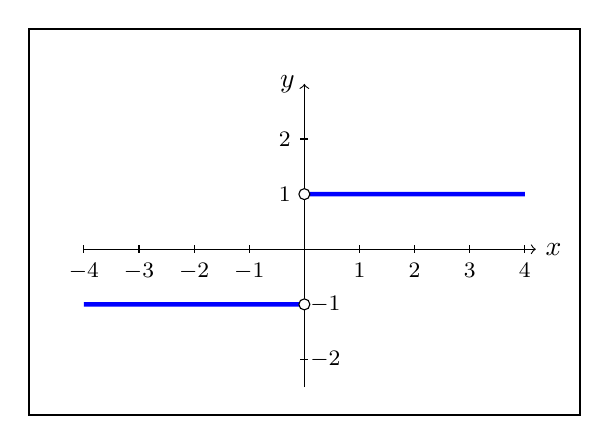
\begin{tikzpicture}[scale=0.7]
	    	% Retangulo em volta
	    	\draw[thick] (-5, -3) rectangle (5, 4);
	    	% Eixos
	    	\draw[->] (-4,0) -- (4.2,0) node[right] {$x$};
	    	\draw[->] (0,-2.5) -- (0, 3) node[left] {$y$};
	    	% Rótulos
	    	\foreach \i in {-4,-3,-2,-1,1,2,3,4}{
	    		\draw (\i,2pt)--(\i, -2pt) node[below]{{\footnotesize $\i$}};
	    	}
	    	\foreach \i in {1,2}{
	    		\draw (2pt,\i)--(-2pt,\i) node[left]{{\footnotesize $\i$}};
	    	}
            \foreach \i in {-2,-1}{
            	\draw (2pt,\i)--(-2pt,\i) node[right]{{\footnotesize $\i$}};
            }    
            \draw[domain=-4:-0.1,ultra thick,variable=\x,blue] plot ({\x},{abs(\x)/\x});
            \draw[domain=0.1:4,ultra thick,variable=\x,blue] plot ({\x},{abs(\x)/\x});
        
            \draw[fill=white] (0,1) circle (0.1);
            \draw[fill=white] (0,-1) circle (0.1);
        
            \end{tikzpicture}
	}{
	    \Fonte{Elaborado pelo autor}
	}	
    \end{figure}    
	\begin{figure}[h!]
		\centering
		\Caption{\label{fig: GrafPartPosFunção f(x) =|x|/x} Gráfico da parte positiva da função $f(x) =\dfrac{|x|}{x}$}	
		\UECEfig{}{
			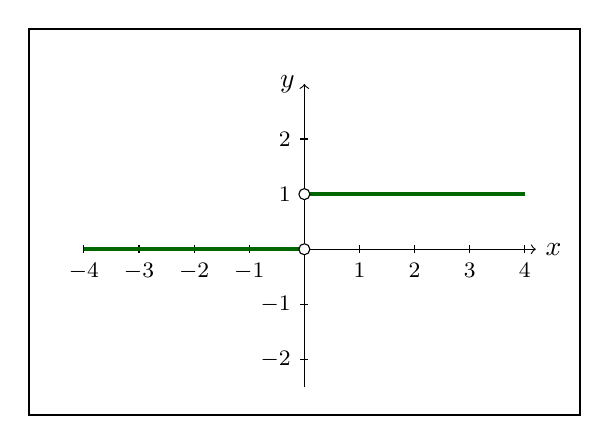
\begin{tikzpicture}[scale=0.7]
				% Retangulo em volta
				\draw[thick] (-5, -3) rectangle (5, 4);
				% Eixos
				\draw[->] (-4,0) -- (4.2,0) node[right] {$x$};
				\draw[->] (0,-2.5) -- (0, 3) node[left] {$y$};
				% Rótulos
				\foreach \i in {-4,-3,-2,-1,1,2,3,4}{
					\draw (\i,2pt)--(\i, -2pt) node[below]{{\footnotesize $\i$}};
				}
				\foreach \i in {-2,-1,1,2}{
					\draw (2pt,\i)--(-2pt,\i) node[left]{{\footnotesize $\i$}};
				}
				
				\draw[domain=-4:-0.1,ultra thick,variable=\x,green!40!black] plot ({\x},{0});
				\draw[domain=0.1:4,ultra thick,variable=\x,green!40!black] plot ({\x},{1});
				
				\draw[fill=white] (0,1) circle (0.1);
				\draw[fill=white] (0,0) circle (0.1);
				
			\end{tikzpicture}
		}{
			\Fonte{Elaborado pelo autor}
		}	
	\end{figure}
\begin{figure}[h!]
	\centering
	\Caption{\label{fig: GrafPartNegFunção f(x) =|x|/x} Gráfico da parte negativa da função $f(x) =\dfrac{|x|}{x}$}
	\UECEfig{}{
		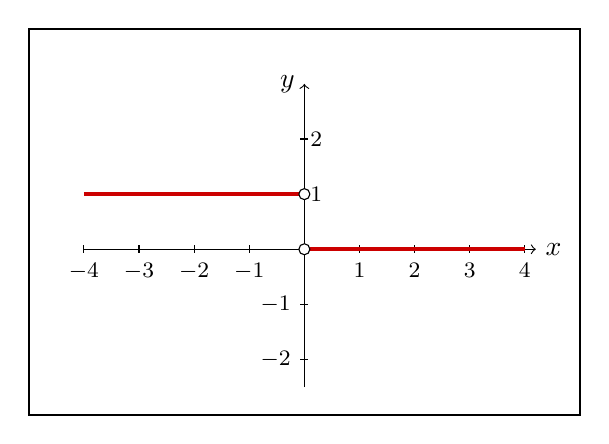
\begin{tikzpicture}[scale=0.7]
			% Retangulo em volta
			\draw[thick] (-5, -3) rectangle (5, 4);
			% Eixos
			\draw[->] (-4,0) -- (4.2,0) node[right] {$x$};
			\draw[->] (0,-2.5) -- (0, 3) node[left] {$y$};
			% Rótulos
			\foreach \i in {-4,-3,-2,-1,1,2,3,4}{
				\draw (\i,2pt)--(\i, -2pt) node[below]{{\footnotesize $\i$}};
			}
			\foreach \i in {1,2}{
				\draw (2pt,\i)--(-2pt,\i) node[right]{{\footnotesize $\i$}};
			}
			\foreach \i in {-2,-1}{
				\draw (2pt,\i)--(-2pt,\i) node[left]{{\footnotesize $\i$}};
			}
			\draw[domain=-4:-0.1,ultra thick,variable=\x,red!80!black] plot ({\x},{1});
			\draw[domain=0.1:4,ultra thick,variable=\x,red!80!black] plot ({\x},{0});
			
			\draw[fill=white] (0,1) circle (0.1);
			\draw[fill=white] (0,0) circle (0.1);
			
		\end{tikzpicture}
	}{
		\Fonte{Elaborado pelo autor}
	}	
\end{figure}

Para finalizarmos esta seção apresentaremos uma relação interessantes sobre uma função mensurável e suas partes positiva e negativa.

    \begin{env}{Lema}
    \label{lem:f = f^+ - f^-}
        Seja $f: X \to \R$ uma função real. Então $f = f^+ - f^-$ e $|f| = f^+ + f^-$.
    \end{env}
    \begin{prova}
            Para provar que $f = f^+ - f^-$, devemos avaliar os casos de $f(x)$. 
            Logo, se $f(x) \geq 0$, então $f^+(x) = \max\{f(x), 0\} = f(x)$ e $f^-(x) = \max\{-f(x), 0\} = 0$, pois $f(x) \geq 0$ implica  $- f(x) \leq~0$.
            Disso, $f^+(x) - f^-(x) = f(x) - 0 = f(x)$, ou seja, $(f^+ - f^-)(x) = f(x)$ tal que $f(x) \geq 0$.
            Caso $f(x) <~0$, então $- f(x) > 0$. 
            Com isso,  $\max\{f(x), 0\} = 0$ e $\max\{-f(x), 0\} = -f(x)$.
            Desta forma vemos que
            $f^+(x) - f^-(x) = 0 - (-f(x)) = f(x)$.
            Em todo caso, $f = f^+ - f^-$.
			Analogamente, se $f(x) \geq 0$, então  $\sup\{f(x), 0\} = f(x)$ e $\sup\{-f(x), 0\} = 0$.
            Assim, $f^+(x) + f^-(x) = f(x)$.
            Caso, $f(x) < 0$, então $ - f(x) > 0$.
            Com isso, obtemos $\sup\{f(x), 0\} = 0$ e $\sup\{-f(x), 0\} = -f(x)$.
            Logo, $f^+(x) + f^-(x) = -f(x)$.
            Desta forma, 
            $$
            (f^+ + f^-)(x) = \max\{f(x), -f(x)\} = |f(x)|.
            $$
            Portanto, $f^+ + f^- = |f|$.
    \end{prova}

Observe que o \ref{lem:f = f^+ - f^-} nos dá a forma das funções $f^+$ e $f^-$ de maneira implícita.
De fato, somando as duas expressões membro a membro vemos que
\vspace{-0.2cm}
$$f + |f| = (f^+ - f^-) + (f^+ + f^-) = 2f^+$$

\vspace{-0.2cm}
Assim, podemos expressar $f^+ = \dfrac{|f| + f}{2}$.
De modo semelhante, conseguimos subtrair membro a membro e obter a expressão $f^- = \dfrac{|f| - f}{2}$. 
Isso demonstra o lema adiante:
\begin{env}{Lema}
\label{lem:forma-explicita-partes-de-uma-funcao}
    Se $f: X \to \R$ é uma função real, então $f^+ = \dfrac{|f| + f}{2}$ e $f^- = \dfrac{|f| - f}{2}$.
    \vspace{-0.2cm}
\end{env}
\begin{env}{Teorema}
    Uma função $f: X \to \R$ é $\cc$-mensurável se, e somente se, suas partes negativa e positiva são ambas $\cc$-mensuráveis. 
    \vspace{-0.2cm}
\end{env}
    \begin{prova}
        Suponha que $f$ seja $\cc$-mensurável.
        Pela  \ref{prop:aritmetica-uma-funcao} vemos que a função $|f|$ é $\cc$-mensurável e pelo \ref{lem:forma-explicita-partes-de-uma-funcao} as funções $f^+ = \dfrac{1}{2}(|f| + f)$ e $f^- = \dfrac{1}{2}(|f| - f)$ também são $\cc$-mensuráveis.
        Reciprocamente, supondo que $f^+$ e $f^-$ são mensuráveis, temos pelo \ref{lem:f = f^+ - f^-} que
        $f = f^+ - f^-$. Segue, novamente pela \ref{prop:aritmetica-duas-funcoes}, que $f$ é $\cc$-mensurável. 
    \end{prova}

Nesta seção, vimos o conceito de $\sigma$-álgebra e, por meio dele, definimos a mensurabilidade de uma função bem como mostramos propriedades disso.
Todos esses conceitos e definições serviram para as seções expostas adiante. 
Na seção seguinte, exploraremos o conceito central deste trabalho: a teoria da medida.´ 